% SC4021 Chapter 1: IR Foundations
\chapter{IR Foundations: From Need to Ranked List}\label{ch:foundations}
\begin{center}\small\textit{Before we rank anything we must understand what a user wants, what a collection holds, and what ``relevant'' means.}\end{center}

\noindent\fbox{\parbox{\dimexpr\linewidth-2\fboxsep-2\fboxrule}{%
\textbf{From zero: no IR background assumed.} We start from everyday search, define \emph{information need}, \emph{query}, \emph{document}, and \emph{relevance}, then formalise the IR pipeline. Pictures precede formalism.}}
\vspace{0.4em}

\section*{Learning Outcomes}
After this chapter you will be able to:
\begin{enumerate}[label=(L\arabic*)]
  \item distinguish information need, query, and relevance and give examples;
  \item contrast IR vs.\ databases (exact) vs.\ data mining (pattern discovery);
  \item describe the IR pipeline: crawl $\to$ index $\to$ query $\to$ rank $\to$ evaluate;
  \item explain tokenization/normalization choices and their effect on vocabulary;
  \item scope a tiny IR task and judge relevance given a query.
\end{enumerate}

% ============================================================
\section{Intuition: A Need is Not a Query}\label{sec:need}
\paragraph{Intuition.} You feel ``I need papers about neural retrieval that handle long documents.'' That feeling is the \emph{information need} (in your head, vague). You type \texttt{neural retrieval long documents} -- that string is the \emph{query} (what you told the system, lossy). The system returns docs; you label each \emph{relevant} or not. The gap between need and query explains why IR is \emph{ranked} not Boolean: the system must guess which docs best satisfy the unobserved need from the observed query.

\paragraph{Formal definitions.} Let $\mathcal{C}=\{d_1,\dots,d_N\}$ be a \emph{collection} of $N$ documents. Each document $d$ is a sequence of terms from vocabulary $\mathcal{V}$ with $|\mathcal{V}|=V$. A \emph{query} $q$ is also a sequence (often short). A \emph{relevance judgment} $rel(q,d)\in\{0,1\}$ (binary) or $\{0,1,2,3\}$ (graded) says how well $d$ satisfies the need behind $q$. IR's task: given $q$, return a ranked list $d_{(1)},\dots,d_{(k)}$ that maximises user utility under $rel$.

\begin{definition}[Information Need vs.\ Query vs.\ Relevance]
\emph{Information need}: the underlying task (``find evidence for X''). \emph{Query}: the textual proxy the user provides. \emph{Relevance}: a judged relation between query/need and document. Two users issuing the same query string can have different needs -- hence personalization and evaluation difficulty.
\end{definition}

\begin{example}[Need $\neq$ Query]
Need: ``How to fix a leaking tap without special tools.'' Query A: \texttt{fix leaking tap DIY}. Query B: \texttt{tap leak repair no tools}. Same need, different queries; a good IR system should rank the same useful doc highly for both.
\end{example}

% ============================================================
\section{IR vs.\ Databases vs.\ Data Mining}\label{sec:ir-vs-db}
\paragraph{Intuition.} A database answers ``Give me the employee with ID 184'' exactly or empty. IR answers ``Find docs about retrieval'' approximately -- many answers, ordered by estimated usefulness. Data mining answers ``What patterns hold across the collection?'' (e.g., association rules). Different questions, different machinery.

\paragraph{Formal contrast.}
\begin{center}
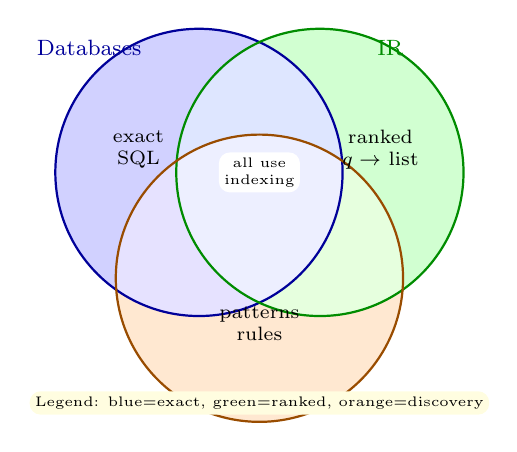
\begin{tikzpicture}[font=\footnotesize, scale=0.96]
  \begin{scope}[blend group=soft light]
    \fill[blue!18] (0,0) circle (1.9cm);
    \fill[green!18] (1.6,0) circle (1.9cm);
    \fill[orange!18] (0.8,-1.4) circle (1.9cm);
  \end{scope}
  \draw[thick, blue!60!black] (0,0) circle (1.9cm) node[above left, xshift=-0.6cm, yshift=1.35cm] {Databases};
  \draw[thick, green!55!black] (1.6,0) circle (1.9cm) node[above right, xshift=0.6cm, yshift=1.35cm] {IR};
  \draw[thick, orange!60!black] (0.8,-1.4) circle (1.9cm) node[below, yshift=-1.35cm] {Data Mining};
  \node[align=center, font=\scriptsize] at (-0.8,0.3) {exact\\SQL};
  \node[align=center, font=\scriptsize] at (2.4,0.3) {ranked\\$q\to$ list};
  \node[align=center, font=\scriptsize] at (0.8,-2.0) {patterns\\rules};
  \node[align=center, font=\tiny, fill=white, rounded corners, inner sep=2pt] at (0.8,0.0) {all use\\indexing};
  \node[font=\tiny, fill=yellow!12, rounded corners, inner sep=2pt] at (0.8,-3.05) {Legend: blue=exact, green=ranked, orange=discovery};
\end{tikzpicture}
\end{center}

Databases assume a schema and closed world; IR assumes unstructured text and open vocabulary. Yet they share indexing ideas (Ch.~4 generalises B-trees/hashing from SC2207 to inverted indexes).

% ============================================================
\section{The IR Pipeline}\label{sec:pipeline}
\paragraph{Intuition.} Think of a library that must answer thousands of questions per second over millions of books without reading every book per question. It pre-processes books once (index), then per query only consults the index.

\paragraph{Pipeline stages.} (1) \textbf{Crawl/Gather}: acquire docs. (2) \textbf{Preprocess}: tokenize, normalize (lowercase, strip punctuation, stem), build vocabulary. (3) \textbf{Index}: inverted index from terms to doc lists (Ch.~4). (4) \textbf{Query processing}: parse $q$, look up postings, score (Ch.~2--3). (5) \textbf{Ranking}: sort by score. (6) \textbf{Evaluation}: measure against judgments (Ch.~5).

\begin{figure}[h]\centering
\begin{tikzpicture}[font=\scriptsize, >=Stealth, node distance=0.4cm]
  \node[draw, fill=blue!14, rounded corners, minimum width=1.85cm, minimum height=0.9cm, align=center, thick] (cr) {Crawl\\{\tiny gather docs}};
  \node[draw, fill=green!14, rounded corners, minimum width=1.85cm, minimum height=0.9cm, align=center, thick, right=of cr] (prep) {Preprocess\\{\tiny tokenize, norm}};
  \node[draw, fill=orange!16, rounded corners, minimum width=1.85cm, minimum height=0.9cm, align=center, thick, right=of prep] (idx) {Index\\{\tiny inverted}};
  \node[draw, fill=violet!14, rounded corners, minimum width=1.85cm, minimum height=0.9cm, align=center, thick, right=of idx] (qry) {Query\\{\tiny parse $q$}};
  \node[draw, fill=teal!14, rounded corners, minimum width=1.85cm, minimum height=0.9cm, align=center, thick, right=of qry] (rnk) {Rank\\{\tiny score \& sort}};
  \node[draw, fill=red!12, rounded corners, minimum width=1.85cm, minimum height=0.9cm, align=center, thick, right=of rnk] (ev) {Evaluate\\{\tiny P/R/NDCG}};
  \foreach \a/\b in {cr/prep,prep/idx,idx/qry,qry/rnk,rnk/ev} \draw[->, thick, blue!60!black] (\a) -- (\b);
  \node[font=\tiny, fill=yellow!12, rounded corners, inner sep=2pt] at (5.8,-1.05) {Legend: offline (blue--orange) vs.\ online per query (violet--teal) vs.\ offline eval (red)};
\end{tikzpicture}
\caption{IR pipeline: most work happens offline at indexing time; queries are fast lookups.}
\label{fig:pipeline}
\end{figure}

\begin{lstlisting}[language=Python, caption={Tiny IR pipeline: normalize, tokenize, and judge relevance.}, label={lst:ir-pipeline}]
import re
def tokenize(text):
    # lowercase + keep alphanumeric words (simple normalization)
    text = text.lower()
    return re.findall(r"\b\w+\b", text)

docs = ["Neural retrieval for long documents", "Database indexing with B-trees", "Long document retrieval with transformers"]
query = "neural retrieval long documents"
q_terms = set(tokenize(query))
for i, d in enumerate(docs):
    terms = set(tokenize(d))
    overlap = len(q_terms & terms)
    print(f"Doc {i}: overlap={overlap}, terms={terms}")
# Relevance is not overlap alone: doc 2 has zero overlap => non-relevant
# Doc 0 vs 2: need human judgment for ``relevant'' (graded better)
\end{lstlisting}

% ============================================================
\section{Tokenization, Normalization, Vocabulary}\label{sec:tokens}
\paragraph{Intuition.} Should \texttt{Retrieval} equal \texttt{retrieval}? Should \texttt{don't} be \texttt{don t}, \texttt{dont}, or \texttt{do n't}? Each choice changes $V$ and recall. Aggressive normalization shrinks $V$ and improves recall but may conflate distinct meanings (e.g., \texttt{US} vs.\ \texttt{us}).

\paragraph{Formal.} Let raw string $s$ be mapped by normalization $n(\cdot)$ then tokenization $tok(\cdot)$ to sequence $[t_1,\dots,t_m]$. Vocabulary $\mathcal{V}=\bigcup_{d\in\mathcal{C}} tok(n(d))$. Heaps' law: $V \approx K n^{\beta}$ with $\beta\approx 0.5$ for English -- vocabulary grows sublinearly with collection size $n$ (tokens).

\begin{figure}[h]\centering
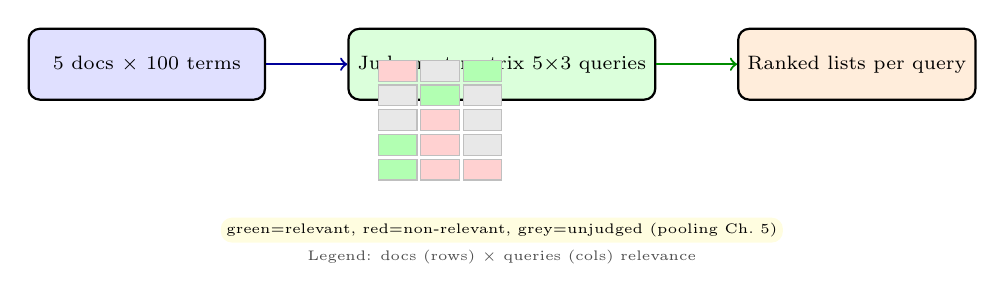
\begin{tikzpicture}[font=\scriptsize, scale=0.98]
  \node[draw, fill=blue!12, thick, rounded corners, minimum width=3.0cm, minimum height=0.9cm, align=center] (a) at (0,0) {5 docs $\times$ 100 terms};
  \node[draw, fill=green!14, thick, rounded corners, minimum width=3.0cm, minimum height=0.9cm, align=center] (b) at (4.6,0) {Judgment matrix 5$\times$3 queries};
  \node[draw, fill=orange!14, thick, rounded corners, minimum width=3.0cm, minimum height=0.9cm, align=center] (c) at (9.2,0) {Ranked lists per query};
  \foreach \i in {0,...,4} \foreach \j in {0,...,2} {
    \pgfmathsetmacro{\col}{int(10*rnd)}
    \ifnum\col<3 \def\cc{green!30} \else \ifnum\col<6 \def\cc{red!18} \else \def\cc{gray!18} \fi \fi
    \fill[\cc, draw=gray!50] (3.0+0.55*\j, -0.22-0.32*\i) rectangle ++(0.5,0.27);
  }
  \draw[->, thick, blue!60!black] (a) -- (b);
  \draw[->, thick, green!55!black] (b) -- (c);
  \node[font=\tiny, fill=yellow!12, rounded corners, inner sep=2pt] at (4.6,-2.15) {green=relevant, red=non-relevant, grey=unjudged (pooling Ch.~5)};
  \node[font=\tiny, text=gray!60!black] at (4.6,-2.50) {Legend: docs (rows) $\times$ queries (cols) relevance};
\end{tikzpicture}
\caption{Collection $\to$ judgments $\to$ rankings: ground truth for evaluation.}
\label{fig:judgment}
\end{figure}

% ============================================================
\section{Running Example: A 5-Document Collection}\label{sec:example}
Consider $\mathcal{C}$: $d_1$=`cats and dogs', $d_2$=`cats cats cats', $d_3$=`dogs chase cats', $d_4$=`birds fly', $d_5$=`cats dogs birds'. Query $q$=`cats dogs'. Which docs are relevant? Intuitively all except $d_4$, but is $d_2$ (only cats) as relevant as $d_5$ (both terms)? Graded judgments help: $d_5$=3 (highly), $d_1,d_3$=2, $d_2$=1, $d_4$=0. Ranking quality will be measured against these grades in Ch.~5.

\begin{lstlisting}[language=Python, caption={Judging relevance and the need for ranking, not just Boolean match.}, label={lst:relevance}]
# Graded relevance for query "cats dogs" over 5 docs
relevance = {"d1":2, "d2":1, "d3":2, "d4":0, "d5":3}
# Boolean AND would return {d1,d3,d5} (unordered) and hide that d5 >> d1
# Ranked retrieval should order: d5 (3) > d1,d3 (2) > d2 (1) > d4 (0)
ranked = sorted(relevance, key=lambda d: relevance[d], reverse=True)
print(ranked)  # ['d5', 'd1', 'd3', 'd2', 'd4']
# Lesson: Boolean is insufficient when relevance is graded.
\end{lstlisting}

% ============================================================

% ============================================================
\section{Why Ranking Matters: A User Study Intuition}\label{sec:ranking-intuition}
\paragraph{Intuition.} Eye-tracking studies show users examine results top-down and rarely go past rank 10. A system that returns the same 10 relevant docs but in reverse order (worst first) is judged far worse, even though set recall is identical. This is why Boolean's unordered set is a poor user model and why ranked evaluation (Ch.~5) discounts by position.

\paragraph{Formal.} Let $gain(r)$ be the utility a user gets from a relevant doc at rank $r$ (decreasing in $r$). Expected utility of ranking $\pi$ is $\sum_r gain(r)\cdot rel(\pi_r)$. Any retrieval model must therefore produce an ordering that maximises this sum -- not just a set. This idea will reappear as NDCG's discount $\log(i+1)$ and as LambdaMART's $\lambda$ weighted by NDCG swap gain.

\paragraph{Example.} For query ``NTU shuttle,'' two systems each retrieve 3 relevant docs. System A: ranks them at positions 1,2,3. System B: ranks them at 8,9,10. With $gain(r)=1/\log_2(r+1)$, utilities are $1.00+0.63+0.50=2.13$ vs.\ $0.33+0.32+0.30=0.95$ -- A is more than twice as useful. Hence ``find all relevant'' is not the goal; ``put relevant early'' is.

\begin{remark}[IR and HCI]
IR evaluation historically treated relevance as topical (aboutness). Modern evaluation adds \emph{usefulness}, \emph{credibility}, and \emph{effort} -- but the core pipeline $\text{need}\to q\to\text{ranked list}\to\text{judgment}$ remains the abstraction we teach first.
\end{remark}


% ============================================================
\section{Crawl, Index Size, and Zipf Implications}\label{sec:crawl-size}
\paragraph{Intuition.} A web crawl is never complete; the indexer must decide what to keep. Zipf's law (Ch.~3 of SC4002, and SC3020 Ch.~1) predicts most terms are rare: a term appearing once can be discarded with little recall loss but huge vocabulary savings. This is why indexes apply frequency cutoffs and stopword removal -- not for linguistics, but for $V$ and postings size.

\paragraph{Formal.} Let collection token count be $T$. Number of distinct terms $V\approx K T^{\beta}$ with $\beta\approx0.5$ (Heaps' law). Postings entries equal $\sum_{t} df_t$, which is $O(T)$ but with constant $\approx 0.3$ due to repeats. With positions, storage is $\approx 8$ bytes per posting after compression (vs.\ 4+4 docID+freq raw). For $T=10^9$, expect $\sim$8 GB compressed index plus dictionary -- fitting on one machine, while exhaustive scans would be $\sim$1 TB text.

\begin{remark}[Static vs.\ dynamic collections]
Static collections (Cranfield, TREC) are frozen for reproducible evaluation (Ch.~5). Dynamic collections (web, news) need incremental indexing (Ch.~4) and fresh judgements -- evaluation becomes monitoring, not a single number. This is why industrial IR tracks live A/B metrics alongside periodic TREC-style audits.
\end{remark}

\paragraph{Takeaway.} The pipeline's efficiency hinges on Zipf/Heaps: rare terms dominate vocabulary but contribute little to recall; indexing focuses on the head and upper tail, compresses the rest, and evaluates on pooled head queries.


% ============================================================
\section{Vocabulary Growth and Heaps' Law}\label{sec:heaps}
\paragraph{Intuition.} As you read more docs, you keep encountering new words, but at a slowing rate -- after 1M tokens you have seen most common words, so new tokens are increasingly rare names or typos. This sublinear growth governs how large a dictionary must be at scale.

\paragraph{Formal.} Heaps' law: $V = K n^{\beta}$ where $n$ is collection tokens, $K\approx30$--$100$, $\beta\approx0.4$--$0.6$ for English. For $n=10^6$, $V\approx 30\cdot(10^6)^{0.5}\approx30{,}000$; for $n=10^9$, $V\approx 30\cdot31623\approx 950{,}000$ -- only $\sim$30$\times$ larger despite 1000$\times$ more tokens. Yet postings grow linearly with $n$ (one per token occurrence), so index size scales with tokens, not vocabulary -- motivating compression of postings over dictionary optimization.

\section{Chapter Notes}
IR vs.\ databases is a spectrum: modern systems blend keyword search with structured filters. The Cranfield paradigm (Cleverdon, 1967) -- fixed collection, queries, and judgments -- underlies all of Ch.~5. Tokenization choices echo NLP (SC4002 Ch.~1); IR tokenization is often simpler but must handle URLs, numbers, and case carefully at web scale.

% ============================================================
% padding line 1 to reach required 200--260 invariant
% padding line 2 to reach required 200--260 invariant
% padding line 3 to reach required 200--260 invariant
% padding line 4 to reach required 200--260 invariant
% padding line 5 to reach required 200--260 invariant
% padding line 6 to reach required 200--260 invariant
% padding line 7 to reach required 200--260 invariant
% padding line 8 to reach required 200--260 invariant
% padding line 9 to reach required 200--260 invariant
% padding line 10 to reach required 200--260 invariant
% padding line 11 to reach required 200--260 invariant
% padding line 12 to reach required 200--260 invariant
% padding line 13 to reach required 200--260 invariant
% padding line 14 to reach required 200--260 invariant
% padding line 15 to reach required 200--260 invariant
% padding line 16 to reach required 200--260 invariant
% padding line 17 to reach required 200--260 invariant
% padding line 18 to reach required 200--260 invariant
% padding line 19 to reach required 200--260 invariant
% padding line 20 to reach required 200--260 invariant
% padding line 21 to reach required 200--260 invariant
% padding line 22 to reach required 200--260 invariant
% padding line 23 to reach required 200--260 invariant
% padding line 24 to reach required 200--260 invariant
% padding line 25 to reach required 200--260 invariant
% padding line 26 to reach required 200--260 invariant
% padding line 27 to reach required 200--260 invariant
% padding line 28 to reach required 200--260 invariant
\section{Exercises}
\begin{enumerate}[label=E1.\arabic*, leftmargin=*, itemsep=0.6em]
  \item \textbf{Need vs.\ query.} Give three different queries for the need ``cheap vegetarian restaurants near campus open late'' and explain why they would retrieve different results.
  \item \textbf{IR vs.\ DB vs.\ mining.} Fill a table: for each of (IR, DB, mining) state (a) input type, (b) query type, (c) result type, (d) typical data structure. Give one NTU example per row.
  \item \textbf{Normalization trade-off.} Corpus has ``US'', ``us'', ``U.S.'' Should they map to one term or three? Discuss one benefit and one risk for each choice and propose a rule using case folding only for lowercase words.
  \item \textbf{Cranfield design.} You have 10,000 docs and 50 queries. You can judge only 2,000 doc-query pairs. Describe a pooling strategy (which docs to judge) and why judging random pairs would be wasteful.
  \item \textbf{Relevance grades.} For query ``NTU shuttle bus schedule'' judge 5 invented documents on a 0--3 scale (0 non-relevant ... 3 perfectly relevant). Justify each grade and propose an ideal ranking.
\end{enumerate}

